\documentclass[hyperref, UTF8, a4paper]{ctexart}

\usepackage{geometry}
\usepackage{titling}
\usepackage{titlesec}
\usepackage{paralist}
\usepackage{footnote}
\usepackage{enumerate}
\usepackage{autobreak}
\usepackage{amsmath, amssymb, amsthm}
\usepackage{mathtools}
\usepackage{bbm}
\usepackage[superscript]{cite}
\usepackage{graphicx}
\usepackage{subfigure}
\usepackage{physics}
\usepackage{siunitx}
\usepackage{tikz}
\usepackage[compat=1.1.0]{tikz-feynhand}
\usepackage[ruled, vlined, linesnumbered, noend]{algorithm2e}
\usepackage{xr-hyper}
\usepackage[colorlinks, linkcolor=black, anchorcolor=black, citecolor=black, filecolor=black]{hyperref}
\usepackage[most]{tcolorbox}
\usepackage{caption}
\usepackage{prettyref}

% Cite: superscript, [1]
\makeatletter
\renewcommand\@citess[1]{\textsuperscript{[#1]}}
\makeatother

\externaldocument[optics-]{../optics/optics}[optics.pdf]
\externaldocument[vasp-]{../cond-comp/vasp/vasp}[vasp.pdf]
\externaldocument[qft-]{../relativistic-qft/relativistic-qft}[relativistic-qft.pdf]
\externaldocument[soft-]{../soft/soft}[soft.pdf]

\geometry{left=3.18cm,right=3.18cm,top=2.54cm,bottom=2.54cm}
\titlespacing{\paragraph}{0pt}{1pt}{10pt}[20pt]
\setlength{\droptitle}{-5em}
\preauthor{\vspace{-10pt}\begin{center}}
\postauthor{\par\end{center}}

\DeclareMathOperator{\timeorder}{\mathcal{T}}
\DeclareMathOperator{\diag}{diag}
\DeclareMathOperator{\legpoly}{P}
\DeclareMathOperator{\primevalue}{P}
\DeclareMathOperator{\sgn}{sgn}
\newcommand*{\ii}{\mathrm{i}}
\newcommand*{\ee}{\mathrm{e}}
\newcommand*{\const}{\mathrm{const}}
\newcommand*{\suchthat}{\quad \text{s.t.} \quad}
\newcommand*{\argmin}{\arg\min}
\newcommand*{\argmax}{\arg\max}
\newcommand*{\normalorder}[1]{: #1 :}
\newcommand*{\pair}[1]{\langle #1 \rangle}
\newcommand*{\fd}[1]{\mathcal{D} #1}

\newrefformat{chap}{第\ref{#1}章}
\newrefformat{sec}{第\ref{#1}节}
\newrefformat{note}{注\ref{#1}}
\newrefformat{fig}{图\ref{#1}}
\newrefformat{alg}{算法\ref{#1}}
\renewcommand{\autoref}{\prettyref}

\usetikzlibrary{arrows,shapes,positioning}
\usetikzlibrary{arrows.meta}
\usetikzlibrary{decorations.markings}
\tikzstyle arrowstyle=[scale=1]
\tikzstyle directed=[postaction={decorate,decoration={markings,
    mark=at position .5 with {\arrow[arrowstyle]{stealth}}}}]
\tikzstyle ray=[directed, thick]
\tikzstyle dot=[anchor=base,fill,circle,inner sep=1pt]

% Algorithm setting
\renewcommand{\algorithmcfname}{算法}
% Python-style code
\SetKwIF{If}{ElseIf}{Else}{if}{:}{elif:}{else:}{}
\SetKwFor{For}{for}{:}{}
\SetKwFor{While}{while}{:}{}
\SetKwInput{KwData}{输入}
\SetKwInput{KwResult}{输出}
\SetArgSty{textnormal}

\tcbuselibrary{skins, breakable, theorems}

\renewcommand{\emph}[1]{\textbf{#1}}
\newcommand*{\concept}[1]{\underline{\textbf{#1}}}

\newcommand{\hmn}[1]{% Hermann-Maguin notation
  \ensuremath{\begingroup\setupHMN #1\endgroup}%
}

\newcommand{\setupHMN}{%
  \doHMN{-}{\HMNoverline}%
  \doHMN{*}{\HMNminverse}%
  \doHMN{i}{\infty}
}

\newcommand{\doHMN}[2]{%
  \begingroup\lccode`~=`#1
  \lowercase{\endgroup\let~}#2%
  \mathcode`#1="8000
}

\newcommand{\HMNminverse}[1]{\frac{#1}{m}}
\newcommand{\HMNoverline}[1]{\mkern1mu\overline{\mkern-1mu#1\mkern-1mu}\mkern1mu}

\newcommand{\Ztwo}{$\mathbb{Z}_2$}

\newcommand{\bigO}[1]{\mathcal{O}(#1)}

\title{准晶的热力学稳定性、生长模式和电子结构}
\author{吴晋渊 18307110155}
\date{}

\begin{document}

\maketitle

\vspace{-3em}

\begin{abstract}
    本文讨论了准晶的形成和性质,分别使用金斯堡-朗道理论讨论了其稳定性以及用相场晶体理论讨论了其生长方式和不同条件下的形貌差异,并回顾了准晶的电子结构。
\end{abstract}

\vspace{3em}

准晶的发现可以追溯到Shechtman等报道的快速冷却的Al-Mn合金的衍射图样中观察到的正二十面体对称性\cite{PhysRevLett.53.1951}。
正二十面体对称性包含一个$C_5$对称轴,而不可能有一个晶格具有这种类型的对称性——它不在晶体允许的32种点群中\cite{Johnston_1960}。
进一步研究表明,他们发现了一个有长程序但没有平移对称性的系统,其长程有序性导致衍射图样上有明锐的斑点,而没有平移对称性意味着其离散旋转对称性不受旋转对称性和晶格必须相容的条件的约束。
这种类型的结构实际上早已被构造出来:它在装饰纹样中有发现\cite{science.1135491},在数学中,彭罗斯镶嵌即为一类典型(但并不唯一)的准晶结构。
此后,大量人工合成的准晶\cite{PhysRevLett.55.511,PhysRevLett.59.1010}和天然形成的准晶陆续被报道\cite{science.1170827}。

准晶有序但无周期性的特殊性质意味着可能可以在其中观察到和普通晶体非常不同的新奇性质,如热学和电学输运性质反常地差\cite{Dolin_ek_2012}。本文简要回顾关于准晶形成和性质的一些议题。\prettyref{sec:gl}通过金斯堡-朗道理论,讨论了准晶序何以能够稳定存在;\prettyref{sec:growth}关于准晶的生长,讨论了不同生长条件下得到的准晶的形貌差异,以及准晶特有的而晶体没有的缺陷产生机制;\prettyref{sec:electron}回顾了准晶的非周期性背景对其中电子行为的影响。

\section{准晶相变的金斯堡-朗道理论}\label{sec:gl}

本节将以文献\cite{PhysRevB.32.5764}为例,介绍准晶相变的金斯堡-朗道理论。
我们采用金斯堡-朗道理论的标准处理方法,假定系统的状态可以使用一个空间中的连续、平滑的序参量描述,系统的行为可以使用一个仅仅关于序参量的自由能完整描述,通过对称性写下自由能的形式,并分析自由能中各参数变动时系统是否发生对称性自发破缺,以及发生后系统基态的性质。
虽然金斯堡-朗道理论通常是用于处理二级相变的,但是如果序参量在两相交界处的变化可以认为比较平缓,从而能够保证系统在相变点附近的行为仍然可以使用一个连续的场论描述,则金斯堡-朗道理论在一级相变中仍然可用(虽然此时标度律等已经失去意义)。使用金斯堡-朗道理论处理固液相变已经成为常见的方法\cite{fabrizio2008,PhysRevB.90.104101}。
事实上,对有明确、不连续的两相交界的一级相变,基于金斯堡-朗道理论的相场方法常常在数值模拟中被使用以避免显式追踪相边界、节约计算资源\cite{provatas2011phase,boettinger2002phase}。

考虑一个具有平移不变性和(连续)旋转不变性的液体。液体结晶属于结构相变,故序参量大体上是密度场。
对一个最一般的系统,序参量选取是否正确、系统自由能是否还依赖于序参量以外的(无法直接从系统的哈密顿量出发获得序参量),但对液体,将自由能写成密度场的一个泛函有理论依据\cite{Evans_2016,cdft2020}。
通常的液体的低能状态是均匀的,而无论是晶体还是准晶依照定义密度分布都不是完全均匀的,如果特定条件下能够形成准晶,那么准晶态必定相较其它状态在某种意义上更加稳定,即系统自由能最低的状态将不再是密度处处为常数的状态。
因此可以将密度场的$\vb*{q} \neq 0$的傅里叶分量$\rho(\vb*{q})$视作结晶的序参量。根据涉及的波矢的个数,液体的自由能的展开式子形如下式:
\begin{equation}
    \begin{aligned}
        F[\rho] &= \sum_\text{all $\vb*{q}$'s} r \rho_{\vb*{q}} \rho_{- \vb*{q}} + u (\rho_{\vb*{q}} \rho_{- \vb*{q}})^2 
        + w \rho_{\vb*{q}} \rho_{- \vb*{q}} \rho_{\vb*{p}} \rho_{- \vb*{p}} 
        + v_3 \rho_{\vb*{q}_1} \rho_{\vb*{q}_2} \rho_{\vb*{q}_3} \delta^3(\vb*{q}_1 + \vb*{q}_2 + \vb*{q}_3) \\
        &\quad \quad + v_4 \rho_{\vb*{q}_1} \rho_{\vb*{q}_2} \rho_{\vb*{q}_3} \rho_{\vb*{q}_4} \delta^3(\sum_i \vb*{q}_i) 
        + v_5 \rho_{\vb*{q}_1} \rho_{\vb*{q}_2} \rho_{\vb*{q}_3} \rho_{\vb*{q}_4} \rho_{\vb*{q}_5}
        \delta^3(\sum_i \vb*{q}_i) + \cdots,
    \end{aligned}
    \label{eq:free-energy-static}
\end{equation}
其中的$\delta$函数保证了理论的空间平移不变性;空间旋转不变性保证了系数仅仅依赖于$\vb*{q}_i$的模长。
据此自由能可以计算$\rho(\vb*{r})$的期望值。如果发现出现非零的$\expval{\rho(\vb*{q})}$意味着出现对称性自发破缺,有某种序形成。
不同种类的序会贡献不同形式的项到$\rho(\vb*{r})$中。例如,一个完美的层列液晶序会贡献一个单独的
\begin{equation}
    \rho_\text{nematic} = \rho(\vb*{q}) (\ee^{\ii \vb*{q} \cdot \vb*{r} + \ii \theta } + \ee^{- \ii \vb*{q} \cdot \vb*{r} - \ii \theta } ) + \rho(2\vb*{q}) (\ee^{\ii \vb*{q} \cdot \vb*{r} + \ii \theta' } + \ee^{- \ii \vb*{q} \cdot \vb*{r} - \ii \theta' } ) + \cdots,
\end{equation}
项,它在一个方向上有连续平移对称性破缺,但是在其它方向上连续平移对称性仍然保持(见\prettyref{fig:smectic})。如果我们只考虑系统的长程行为,可以截断高次谐波。
使用$\rho(\vb*{q})$的语言,就是由液晶序贡献的那部分密度中有$\rho(\vb*{q}) = \text{phase factor} \times \rho(-\vb*{q})$,其中$\vb*{q}$方向取为液晶分子的指向,长度取为$2\pi n/ L$,因为液晶仍然保留了$C_2$对称性。这里$\theta$因子来自液晶序可以整体平移这一事实。
类似的,一个保留了$C_3$对称性的序中$\rho(\vb*{q}_1)$, $\rho(\vb*{q}_2)$, $\rho(\vb*{q}_3)$这三个量也只应该相差一个相因子,其中$\vb*{q}_2$是$\vb*{q}_1$绕着指定的轴旋转\SI{120}{\degree}得到的矢量,$\vb*{q}_3$是$\vb*{q}_1$绕着同一个轴旋转\SI{240}{\degree}得到的;$\rho(\vb*{q}_1)$, $\rho(\vb*{q}_2)$, $\rho(\vb*{q}_3)$这三个量的相位因子来自序中原子的平移,它们相差的相位因子则表明了$C_3$序的晶格常数。
因此,通过观察$\rho(\vb*{q})$的不同成分可以辨认出体系中的不同序。

\begin{figure}
    \centering
    

\tikzset{every picture/.style={line width=0.75pt}} %set default line width to 0.75pt        

\begin{tikzpicture}[x=0.75pt,y=0.75pt,yscale=-0.7,xscale=0.7]
%uncomment if require: \path (0,300); %set diagram left start at 0, and has height of 300

%Rounded Rect [id:dp05563000442277022] 
\draw  [fill={rgb, 255:red, 255; green, 255; blue, 255 }  ,fill opacity=1 ] (137,200.08) .. controls (138.7,200.08) and (140.08,198.7) .. (140.08,197) -- (140.08,170.33) .. controls (140.08,168.63) and (138.7,167.25) .. (137,167.25) -- (137,167.25) .. controls (135.3,167.25) and (133.92,168.63) .. (133.92,170.33) -- (133.92,197) .. controls (133.92,198.7) and (135.3,200.08) .. (137,200.08) -- cycle ;
%Rounded Rect [id:dp6531641548320384] 
\draw  [fill={rgb, 255:red, 255; green, 255; blue, 255 }  ,fill opacity=1 ] (144.17,200.08) .. controls (145.87,200.08) and (147.25,198.7) .. (147.25,197) -- (147.25,170.33) .. controls (147.25,168.63) and (145.87,167.25) .. (144.17,167.25) -- (144.17,167.25) .. controls (142.46,167.25) and (141.08,168.63) .. (141.08,170.33) -- (141.08,197) .. controls (141.08,198.7) and (142.46,200.08) .. (144.17,200.08) -- cycle ;
%Rounded Rect [id:dp7705246921925859] 
\draw  [fill={rgb, 255:red, 255; green, 255; blue, 255 }  ,fill opacity=1 ] (150.33,200.08) .. controls (152.04,200.08) and (153.42,198.7) .. (153.42,197) -- (153.42,170.33) .. controls (153.42,168.63) and (152.04,167.25) .. (150.33,167.25) -- (150.33,167.25) .. controls (148.63,167.25) and (147.25,168.63) .. (147.25,170.33) -- (147.25,197) .. controls (147.25,198.7) and (148.63,200.08) .. (150.33,200.08) -- cycle ;
%Rounded Rect [id:dp16514777594403607] 
\draw  [fill={rgb, 255:red, 255; green, 255; blue, 255 }  ,fill opacity=1 ] (180.33,194.92) .. controls (182.04,194.92) and (183.42,193.54) .. (183.42,191.83) -- (183.42,165.17) .. controls (183.42,163.46) and (182.04,162.08) .. (180.33,162.08) -- (180.33,162.08) .. controls (178.63,162.08) and (177.25,163.46) .. (177.25,165.17) -- (177.25,191.83) .. controls (177.25,193.54) and (178.63,194.92) .. (180.33,194.92) -- cycle ;
%Rounded Rect [id:dp9545252921582017] 
\draw  [fill={rgb, 255:red, 255; green, 255; blue, 255 }  ,fill opacity=1 ] (183.17,204.08) .. controls (184.87,204.08) and (186.25,202.7) .. (186.25,201) -- (186.25,174.33) .. controls (186.25,172.63) and (184.87,171.25) .. (183.17,171.25) -- (183.17,171.25) .. controls (181.46,171.25) and (180.08,172.63) .. (180.08,174.33) -- (180.08,201) .. controls (180.08,202.7) and (181.46,204.08) .. (183.17,204.08) -- cycle ;
%Rounded Rect [id:dp6380802078932455] 
\draw  [fill={rgb, 255:red, 255; green, 255; blue, 255 }  ,fill opacity=1 ] (192.17,194.08) .. controls (193.87,194.08) and (195.25,192.7) .. (195.25,191) -- (195.25,164.33) .. controls (195.25,162.63) and (193.87,161.25) .. (192.17,161.25) -- (192.17,161.25) .. controls (190.46,161.25) and (189.08,162.63) .. (189.08,164.33) -- (189.08,191) .. controls (189.08,192.7) and (190.46,194.08) .. (192.17,194.08) -- cycle ;
%Rounded Rect [id:dp49673386562771316] 
\draw  [fill={rgb, 255:red, 255; green, 255; blue, 255 }  ,fill opacity=1 ] (161.17,198.08) .. controls (162.87,198.08) and (164.25,196.7) .. (164.25,195) -- (164.25,168.33) .. controls (164.25,166.63) and (162.87,165.25) .. (161.17,165.25) -- (161.17,165.25) .. controls (159.46,165.25) and (158.08,166.63) .. (158.08,168.33) -- (158.08,195) .. controls (158.08,196.7) and (159.46,198.08) .. (161.17,198.08) -- cycle ;
%Rounded Rect [id:dp944726253294734] 
\draw  [fill={rgb, 255:red, 255; green, 255; blue, 255 }  ,fill opacity=1 ] (178.17,196.92) .. controls (179.87,196.92) and (181.25,195.54) .. (181.25,193.83) -- (181.25,167.17) .. controls (181.25,165.46) and (179.87,164.08) .. (178.17,164.08) -- (178.17,164.08) .. controls (176.46,164.08) and (175.08,165.46) .. (175.08,167.17) -- (175.08,193.83) .. controls (175.08,195.54) and (176.46,196.92) .. (178.17,196.92) -- cycle ;
%Rounded Rect [id:dp7634948824752461] 
\draw  [fill={rgb, 255:red, 255; green, 255; blue, 255 }  ,fill opacity=1 ] (164.25,201.17) .. controls (165.95,201.17) and (167.33,199.79) .. (167.33,198.08) -- (167.33,171.42) .. controls (167.33,169.71) and (165.95,168.33) .. (164.25,168.33) -- (164.25,168.33) .. controls (162.55,168.33) and (161.17,169.71) .. (161.17,171.42) -- (161.17,198.08) .. controls (161.17,199.79) and (162.55,201.17) .. (164.25,201.17) -- cycle ;
%Rounded Rect [id:dp842642877347413] 
\draw  [fill={rgb, 255:red, 255; green, 255; blue, 255 }  ,fill opacity=1 ] (204.17,194.08) .. controls (205.87,194.08) and (207.25,192.7) .. (207.25,191) -- (207.25,164.33) .. controls (207.25,162.63) and (205.87,161.25) .. (204.17,161.25) -- (204.17,161.25) .. controls (202.46,161.25) and (201.08,162.63) .. (201.08,164.33) -- (201.08,191) .. controls (201.08,192.7) and (202.46,194.08) .. (204.17,194.08) -- cycle ;
%Rounded Rect [id:dp2527241147768988] 
\draw  [fill={rgb, 255:red, 255; green, 255; blue, 255 }  ,fill opacity=1 ] (215,192.08) .. controls (216.7,192.08) and (218.08,190.7) .. (218.08,189) -- (218.08,162.33) .. controls (218.08,160.63) and (216.7,159.25) .. (215,159.25) -- (215,159.25) .. controls (213.3,159.25) and (211.92,160.63) .. (211.92,162.33) -- (211.92,189) .. controls (211.92,190.7) and (213.3,192.08) .. (215,192.08) -- cycle ;
%Rounded Rect [id:dp10611436324219059] 
\draw  [fill={rgb, 255:red, 255; green, 255; blue, 255 }  ,fill opacity=1 ] (221.17,192.08) .. controls (222.87,192.08) and (224.25,190.7) .. (224.25,189) -- (224.25,162.33) .. controls (224.25,160.63) and (222.87,159.25) .. (221.17,159.25) -- (221.17,159.25) .. controls (219.46,159.25) and (218.08,160.63) .. (218.08,162.33) -- (218.08,189) .. controls (218.08,190.7) and (219.46,192.08) .. (221.17,192.08) -- cycle ;
%Rounded Rect [id:dp6761737981434759] 
\draw  [fill={rgb, 255:red, 255; green, 255; blue, 255 }  ,fill opacity=1 ] (138,128.08) .. controls (139.7,128.08) and (141.08,126.7) .. (141.08,125) -- (141.08,98.33) .. controls (141.08,96.63) and (139.7,95.25) .. (138,95.25) -- (138,95.25) .. controls (136.3,95.25) and (134.92,96.63) .. (134.92,98.33) -- (134.92,125) .. controls (134.92,126.7) and (136.3,128.08) .. (138,128.08) -- cycle ;
%Rounded Rect [id:dp44018912567548596] 
\draw  [fill={rgb, 255:red, 255; green, 255; blue, 255 }  ,fill opacity=1 ] (145.17,128.08) .. controls (146.87,128.08) and (148.25,126.7) .. (148.25,125) -- (148.25,98.33) .. controls (148.25,96.63) and (146.87,95.25) .. (145.17,95.25) -- (145.17,95.25) .. controls (143.46,95.25) and (142.08,96.63) .. (142.08,98.33) -- (142.08,125) .. controls (142.08,126.7) and (143.46,128.08) .. (145.17,128.08) -- cycle ;
%Rounded Rect [id:dp049822785616503884] 
\draw  [fill={rgb, 255:red, 255; green, 255; blue, 255 }  ,fill opacity=1 ] (151.33,128.08) .. controls (153.04,128.08) and (154.42,126.7) .. (154.42,125) -- (154.42,98.33) .. controls (154.42,96.63) and (153.04,95.25) .. (151.33,95.25) -- (151.33,95.25) .. controls (149.63,95.25) and (148.25,96.63) .. (148.25,98.33) -- (148.25,125) .. controls (148.25,126.7) and (149.63,128.08) .. (151.33,128.08) -- cycle ;
%Rounded Rect [id:dp7275156706152337] 
\draw  [fill={rgb, 255:red, 255; green, 255; blue, 255 }  ,fill opacity=1 ] (181.33,122.92) .. controls (183.04,122.92) and (184.42,121.54) .. (184.42,119.83) -- (184.42,93.17) .. controls (184.42,91.46) and (183.04,90.08) .. (181.33,90.08) -- (181.33,90.08) .. controls (179.63,90.08) and (178.25,91.46) .. (178.25,93.17) -- (178.25,119.83) .. controls (178.25,121.54) and (179.63,122.92) .. (181.33,122.92) -- cycle ;
%Rounded Rect [id:dp7851150622633405] 
\draw  [fill={rgb, 255:red, 255; green, 255; blue, 255 }  ,fill opacity=1 ] (184.17,132.08) .. controls (185.87,132.08) and (187.25,130.7) .. (187.25,129) -- (187.25,102.33) .. controls (187.25,100.63) and (185.87,99.25) .. (184.17,99.25) -- (184.17,99.25) .. controls (182.46,99.25) and (181.08,100.63) .. (181.08,102.33) -- (181.08,129) .. controls (181.08,130.7) and (182.46,132.08) .. (184.17,132.08) -- cycle ;
%Rounded Rect [id:dp023929054330812827] 
\draw  [fill={rgb, 255:red, 255; green, 255; blue, 255 }  ,fill opacity=1 ] (193.17,122.08) .. controls (194.87,122.08) and (196.25,120.7) .. (196.25,119) -- (196.25,92.33) .. controls (196.25,90.63) and (194.87,89.25) .. (193.17,89.25) -- (193.17,89.25) .. controls (191.46,89.25) and (190.08,90.63) .. (190.08,92.33) -- (190.08,119) .. controls (190.08,120.7) and (191.46,122.08) .. (193.17,122.08) -- cycle ;
%Rounded Rect [id:dp8807448370596598] 
\draw  [fill={rgb, 255:red, 255; green, 255; blue, 255 }  ,fill opacity=1 ] (162.17,126.08) .. controls (163.87,126.08) and (165.25,124.7) .. (165.25,123) -- (165.25,96.33) .. controls (165.25,94.63) and (163.87,93.25) .. (162.17,93.25) -- (162.17,93.25) .. controls (160.46,93.25) and (159.08,94.63) .. (159.08,96.33) -- (159.08,123) .. controls (159.08,124.7) and (160.46,126.08) .. (162.17,126.08) -- cycle ;
%Rounded Rect [id:dp2406222646847067] 
\draw  [fill={rgb, 255:red, 255; green, 255; blue, 255 }  ,fill opacity=1 ] (179.17,124.92) .. controls (180.87,124.92) and (182.25,123.54) .. (182.25,121.83) -- (182.25,95.17) .. controls (182.25,93.46) and (180.87,92.08) .. (179.17,92.08) -- (179.17,92.08) .. controls (177.46,92.08) and (176.08,93.46) .. (176.08,95.17) -- (176.08,121.83) .. controls (176.08,123.54) and (177.46,124.92) .. (179.17,124.92) -- cycle ;
%Rounded Rect [id:dp8366661122103913] 
\draw  [fill={rgb, 255:red, 255; green, 255; blue, 255 }  ,fill opacity=1 ] (165.25,129.17) .. controls (166.95,129.17) and (168.33,127.79) .. (168.33,126.08) -- (168.33,99.42) .. controls (168.33,97.71) and (166.95,96.33) .. (165.25,96.33) -- (165.25,96.33) .. controls (163.55,96.33) and (162.17,97.71) .. (162.17,99.42) -- (162.17,126.08) .. controls (162.17,127.79) and (163.55,129.17) .. (165.25,129.17) -- cycle ;
%Rounded Rect [id:dp5979480085184197] 
\draw  [fill={rgb, 255:red, 255; green, 255; blue, 255 }  ,fill opacity=1 ] (205.17,122.08) .. controls (206.87,122.08) and (208.25,120.7) .. (208.25,119) -- (208.25,92.33) .. controls (208.25,90.63) and (206.87,89.25) .. (205.17,89.25) -- (205.17,89.25) .. controls (203.46,89.25) and (202.08,90.63) .. (202.08,92.33) -- (202.08,119) .. controls (202.08,120.7) and (203.46,122.08) .. (205.17,122.08) -- cycle ;
%Rounded Rect [id:dp5520431708688049] 
\draw  [fill={rgb, 255:red, 255; green, 255; blue, 255 }  ,fill opacity=1 ] (216,120.08) .. controls (217.7,120.08) and (219.08,118.7) .. (219.08,117) -- (219.08,90.33) .. controls (219.08,88.63) and (217.7,87.25) .. (216,87.25) -- (216,87.25) .. controls (214.3,87.25) and (212.92,88.63) .. (212.92,90.33) -- (212.92,117) .. controls (212.92,118.7) and (214.3,120.08) .. (216,120.08) -- cycle ;
%Rounded Rect [id:dp9248678649410391] 
\draw  [fill={rgb, 255:red, 255; green, 255; blue, 255 }  ,fill opacity=1 ] (222.17,120.08) .. controls (223.87,120.08) and (225.25,118.7) .. (225.25,117) -- (225.25,90.33) .. controls (225.25,88.63) and (223.87,87.25) .. (222.17,87.25) -- (222.17,87.25) .. controls (220.46,87.25) and (219.08,88.63) .. (219.08,90.33) -- (219.08,117) .. controls (219.08,118.7) and (220.46,120.08) .. (222.17,120.08) -- cycle ;
%Rounded Rect [id:dp11633727618214662] 
\draw  [fill={rgb, 255:red, 255; green, 255; blue, 255 }  ,fill opacity=1 ] (133,272.08) .. controls (134.7,272.08) and (136.08,270.7) .. (136.08,269) -- (136.08,242.33) .. controls (136.08,240.63) and (134.7,239.25) .. (133,239.25) -- (133,239.25) .. controls (131.3,239.25) and (129.92,240.63) .. (129.92,242.33) -- (129.92,269) .. controls (129.92,270.7) and (131.3,272.08) .. (133,272.08) -- cycle ;
%Rounded Rect [id:dp19991605793380307] 
\draw  [fill={rgb, 255:red, 255; green, 255; blue, 255 }  ,fill opacity=1 ] (140.17,272.08) .. controls (141.87,272.08) and (143.25,270.7) .. (143.25,269) -- (143.25,242.33) .. controls (143.25,240.63) and (141.87,239.25) .. (140.17,239.25) -- (140.17,239.25) .. controls (138.46,239.25) and (137.08,240.63) .. (137.08,242.33) -- (137.08,269) .. controls (137.08,270.7) and (138.46,272.08) .. (140.17,272.08) -- cycle ;
%Rounded Rect [id:dp42844763551577003] 
\draw  [fill={rgb, 255:red, 255; green, 255; blue, 255 }  ,fill opacity=1 ] (146.33,272.08) .. controls (148.04,272.08) and (149.42,270.7) .. (149.42,269) -- (149.42,242.33) .. controls (149.42,240.63) and (148.04,239.25) .. (146.33,239.25) -- (146.33,239.25) .. controls (144.63,239.25) and (143.25,240.63) .. (143.25,242.33) -- (143.25,269) .. controls (143.25,270.7) and (144.63,272.08) .. (146.33,272.08) -- cycle ;
%Rounded Rect [id:dp39463105589249836] 
\draw  [fill={rgb, 255:red, 255; green, 255; blue, 255 }  ,fill opacity=1 ] (176.33,266.92) .. controls (178.04,266.92) and (179.42,265.54) .. (179.42,263.83) -- (179.42,237.17) .. controls (179.42,235.46) and (178.04,234.08) .. (176.33,234.08) -- (176.33,234.08) .. controls (174.63,234.08) and (173.25,235.46) .. (173.25,237.17) -- (173.25,263.83) .. controls (173.25,265.54) and (174.63,266.92) .. (176.33,266.92) -- cycle ;
%Rounded Rect [id:dp5570828347495911] 
\draw  [fill={rgb, 255:red, 255; green, 255; blue, 255 }  ,fill opacity=1 ] (179.17,276.08) .. controls (180.87,276.08) and (182.25,274.7) .. (182.25,273) -- (182.25,246.33) .. controls (182.25,244.63) and (180.87,243.25) .. (179.17,243.25) -- (179.17,243.25) .. controls (177.46,243.25) and (176.08,244.63) .. (176.08,246.33) -- (176.08,273) .. controls (176.08,274.7) and (177.46,276.08) .. (179.17,276.08) -- cycle ;
%Rounded Rect [id:dp8351877025940617] 
\draw  [fill={rgb, 255:red, 255; green, 255; blue, 255 }  ,fill opacity=1 ] (188.17,266.08) .. controls (189.87,266.08) and (191.25,264.7) .. (191.25,263) -- (191.25,236.33) .. controls (191.25,234.63) and (189.87,233.25) .. (188.17,233.25) -- (188.17,233.25) .. controls (186.46,233.25) and (185.08,234.63) .. (185.08,236.33) -- (185.08,263) .. controls (185.08,264.7) and (186.46,266.08) .. (188.17,266.08) -- cycle ;
%Rounded Rect [id:dp8163905794152979] 
\draw  [fill={rgb, 255:red, 255; green, 255; blue, 255 }  ,fill opacity=1 ] (157.17,270.08) .. controls (158.87,270.08) and (160.25,268.7) .. (160.25,267) -- (160.25,240.33) .. controls (160.25,238.63) and (158.87,237.25) .. (157.17,237.25) -- (157.17,237.25) .. controls (155.46,237.25) and (154.08,238.63) .. (154.08,240.33) -- (154.08,267) .. controls (154.08,268.7) and (155.46,270.08) .. (157.17,270.08) -- cycle ;
%Rounded Rect [id:dp021154523060017638] 
\draw  [fill={rgb, 255:red, 255; green, 255; blue, 255 }  ,fill opacity=1 ] (174.17,268.92) .. controls (175.87,268.92) and (177.25,267.54) .. (177.25,265.83) -- (177.25,239.17) .. controls (177.25,237.46) and (175.87,236.08) .. (174.17,236.08) -- (174.17,236.08) .. controls (172.46,236.08) and (171.08,237.46) .. (171.08,239.17) -- (171.08,265.83) .. controls (171.08,267.54) and (172.46,268.92) .. (174.17,268.92) -- cycle ;
%Rounded Rect [id:dp6107290134756147] 
\draw  [fill={rgb, 255:red, 255; green, 255; blue, 255 }  ,fill opacity=1 ] (160.25,273.17) .. controls (161.95,273.17) and (163.33,271.79) .. (163.33,270.08) -- (163.33,243.42) .. controls (163.33,241.71) and (161.95,240.33) .. (160.25,240.33) -- (160.25,240.33) .. controls (158.55,240.33) and (157.17,241.71) .. (157.17,243.42) -- (157.17,270.08) .. controls (157.17,271.79) and (158.55,273.17) .. (160.25,273.17) -- cycle ;
%Rounded Rect [id:dp6749271405762176] 
\draw  [fill={rgb, 255:red, 255; green, 255; blue, 255 }  ,fill opacity=1 ] (200.17,266.08) .. controls (201.87,266.08) and (203.25,264.7) .. (203.25,263) -- (203.25,236.33) .. controls (203.25,234.63) and (201.87,233.25) .. (200.17,233.25) -- (200.17,233.25) .. controls (198.46,233.25) and (197.08,234.63) .. (197.08,236.33) -- (197.08,263) .. controls (197.08,264.7) and (198.46,266.08) .. (200.17,266.08) -- cycle ;
%Rounded Rect [id:dp9946230417394801] 
\draw  [fill={rgb, 255:red, 255; green, 255; blue, 255 }  ,fill opacity=1 ] (211,264.08) .. controls (212.7,264.08) and (214.08,262.7) .. (214.08,261) -- (214.08,234.33) .. controls (214.08,232.63) and (212.7,231.25) .. (211,231.25) -- (211,231.25) .. controls (209.3,231.25) and (207.92,232.63) .. (207.92,234.33) -- (207.92,261) .. controls (207.92,262.7) and (209.3,264.08) .. (211,264.08) -- cycle ;
%Rounded Rect [id:dp15697973709097868] 
\draw  [fill={rgb, 255:red, 255; green, 255; blue, 255 }  ,fill opacity=1 ] (217.17,264.08) .. controls (218.87,264.08) and (220.25,262.7) .. (220.25,261) -- (220.25,234.33) .. controls (220.25,232.63) and (218.87,231.25) .. (217.17,231.25) -- (217.17,231.25) .. controls (215.46,231.25) and (214.08,232.63) .. (214.08,234.33) -- (214.08,261) .. controls (214.08,262.7) and (215.46,264.08) .. (217.17,264.08) -- cycle ;
%Straight Lines [id:da5282684837420737] 
\draw    (70,176) -- (70,113.33) ;
\draw [shift={(70,111.33)}, rotate = 90] [color={rgb, 255:red, 0; green, 0; blue, 0 }  ][line width=0.75]    (10.93,-3.29) .. controls (6.95,-1.4) and (3.31,-0.3) .. (0,0) .. controls (3.31,0.3) and (6.95,1.4) .. (10.93,3.29)   ;
%Straight Lines [id:da8123690998660977] 
\draw    (238,283) -- (403,283) ;
\draw [shift={(405,283)}, rotate = 180] [fill={rgb, 255:red, 0; green, 0; blue, 0 }  ][line width=0.08]  [draw opacity=0] (12,-3) -- (0,0) -- (12,3) -- cycle    ;
%Straight Lines [id:da7045381375059749] 
\draw    (238,283) -- (238,60.33) ;
\draw [shift={(238,58.33)}, rotate = 90] [fill={rgb, 255:red, 0; green, 0; blue, 0 }  ][line width=0.08]  [draw opacity=0] (12,-3) -- (0,0) -- (12,3) -- cycle    ;
%Shape: Wave [id:dp6487755568120255] 
\draw   (272.03,62.33) .. controls (253.33,65.86) and (240,69.44) .. (240,73.37) .. controls (240,79.62) and (273.65,85) .. (309,90.62) .. controls (344.35,96.25) and (378,101.63) .. (378,107.87) .. controls (378,114.12) and (344.35,119.5) .. (309,125.12) .. controls (273.65,130.75) and (240,136.13) .. (240,142.37) .. controls (240,148.62) and (273.65,154) .. (309,159.62) .. controls (344.35,165.25) and (378,170.63) .. (378,176.87) .. controls (378,183.12) and (344.35,188.5) .. (309,194.12) .. controls (273.65,199.75) and (240,205.13) .. (240,211.37) .. controls (240,217.62) and (273.65,223) .. (309,228.62) .. controls (344.35,234.25) and (378,239.63) .. (378,245.87) .. controls (378,252.12) and (344.35,257.5) .. (309,263.12) .. controls (273.65,268.75) and (240,274.13) .. (240,280.37) .. controls (240,281.38) and (240.88,282.37) .. (242.5,283.33) ;

% Text Node
\draw (70,107.93) node [anchor=south] [inner sep=0.75pt]    {$\boldsymbol{q}$};
% Text Node
\draw (407,283) node [anchor=west] [inner sep=0.75pt]   [align=left] {density};


\end{tikzpicture}

    \caption{层状液晶的密度分布:一个方向上出现了空间平移对称性破缺,从而有一个波矢,但是其它方向上密度仍然是大体上均匀的}
    \label{fig:smectic}
\end{figure}

\begin{figure}
    \centering
    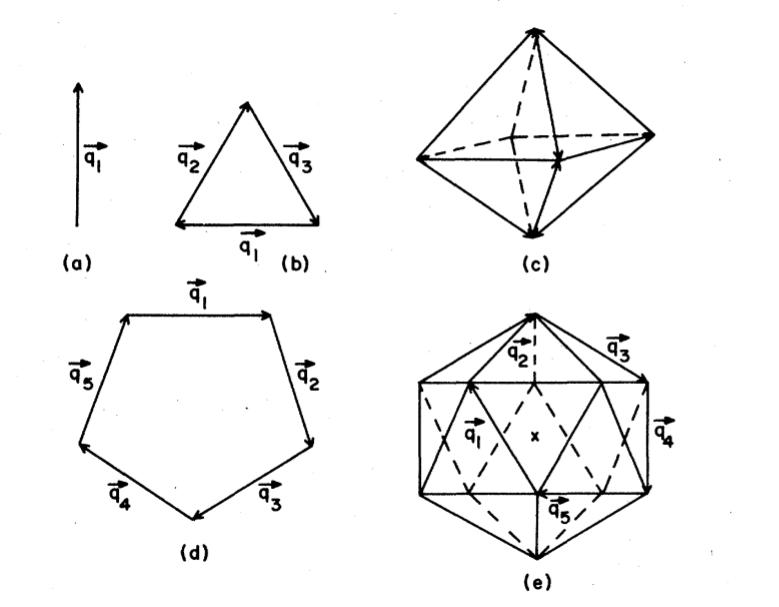
\includegraphics[width=0.6\textwidth]{wavevector.PNG}
    \caption{文献\cite{PhysRevB.32.5764}中的图1,不同序的密度场的非零傅里叶分量的波矢。(a) 简单的层状液晶,(b) 三棱柱状液晶,(c) 体心立方晶格,具有正八面体对称性,图中标出了六个独立的波矢方向,(d) 五棱柱状液晶,在$z$方向上没有破缺平移对称性,但是在$xy$平面上构成彭罗斯镶嵌(e) 正二十面体对称性的准晶}
    \label{fig:wavevectors}
\end{figure}

容易看出,由于\eqref{eq:free-energy-static}中各项都有$\delta$函数,只有对称性匹配的序才能对\eqref{eq:free-energy-static}中的特定一项有贡献。
以下为简便起见,我们考虑一个液体,在其中$v_4$不重要,只有$v_3$和$v_5$项是重要的。显然,如果某种序中能够找到三个波矢和为零的傅里叶分量,那么这个序会对$v_3$项有贡献,否则就没有贡献。一个体心立方晶格(bcc)的点群是$O_h$,从而其对称性和正八面体完全相同;空间群在波矢上的作用仅有点群操作有非平庸的效果,因此一个bcc序对密度的贡献中,所有的波矢都可以放在一个正八面体的棱上,即
\begin{equation}
    \rho(\vb*{r}) = \sum_\text{$\vb*{q}_i$ in octahedron edge} \frac{\rho}{\sqrt{6}} \cos(\vb*{q}_i \cdot \vb*{r} + \theta_i) + \cdots,
\end{equation}
其中$\cdots$指的是bcc格点的内部结构导致的高次谐波,此处略去;一个正八面体有12条棱,但是为了保证空间倒转对称性,我们需要让正对的两条棱上的波矢符号相反,因此只需要求和6条棱;这里我们已经将$\vb*{q}_i$和$-\vb*{q}_i$项的贡献加了起来,并且做了正确的归一化。
计算得到最低的自由能为
\begin{equation}
    (F_3)_\text{min} = - \frac{2 \rho^3 v_3}{3 \sqrt{6}}.
    \label{eq:bcc-free-energy}
\end{equation}
另一种对$v_3$项有贡献的序是截面为三角形的棒状液晶,但是由于一个正八面体中有更多首尾相连构成三角形的波矢,一般来说这种棒状液晶不如bcc稳定。

类似的,$v_5$项只能由一个波矢中有五个波矢能够首尾相连成五边形的序“激活”,如具有$C_5$对称性的序。注意这个序不是周期的,因为五个波矢不可公度,但是既然我们是在讨论平滑化的场,没有周期性毫无影响。一种可能的序是截面为五边形的棱柱状液晶,在$z$轴上是比较连续的,但是在$xy$平面上是非周期性密铺,其波矢结构如\prettyref{fig:wavevectors}(d),密度场为
\begin{equation}
    \rho(\boldsymbol{r})=\sum_{i=1}^{5} \frac{\rho}{\sqrt{5}} \cos \left(\boldsymbol{q}_{i} \cdot \boldsymbol{r}+\theta_{i}\right),
\end{equation}
其自由能的极小值为
\begin{equation}
    (F_{5})_\text{min} =-\frac{v_{5}}{25 \sqrt{5}} \rho^{5}.
    \label{eq:rodlike-lyotropic-free-energy}
\end{equation}

还有一个更加结构更加复杂的序能够同时激活$v_3$项和$v_5$项:波矢结构为\prettyref{fig:wavevectors}(e)中的正二十面体的准晶。
可以看到,\prettyref{fig:wavevectors}(e)中的波矢既能够形成首尾相连的三角形,也能够形成首尾相连的五边形,因此对$v_3$项和$v_5$项都有贡献。
与前述两个序类似,可以计算出这种准晶序的最低的自由能是
\begin{equation}
    \left(F_{3}+F_{5}\right)_{\min }=-\frac{2 \rho^{3} v_{3}}{75 \sqrt{15}}-\frac{2 \rho^{5} v_{5}}{3 \sqrt{15}}.
    \label{eq:quasi-crystal-free-energy}
\end{equation}
比较\eqref{eq:bcc-free-energy},\eqref{eq:rodlike-lyotropic-free-energy}和\eqref{eq:quasi-crystal-free-energy},可以发现\eqref{eq:quasi-crystal-free-energy}总是低于\eqref{eq:rodlike-lyotropic-free-energy},即准晶序总是比五棱柱液晶序稳定,但是\eqref{eq:bcc-free-energy}和\eqref{eq:quasi-crystal-free-energy}的大小关系在$v_3$和$v_5$值没有给定时是不能确定的。
因此,调节$v_3$和$v_5$项,可以让正二十面体对称性的准晶序和正八面体对称性的bcc晶体序互相转化。

综上所述,我们可以看到,在结晶过程的金斯堡-朗道理论描述中,准晶序除了对称性和晶体序不同以外,其它没有任何不同;没有什么对称性上条件要求\eqref{eq:free-energy-static}中不能出现$v_5$之类的项,而有这种项出现,准晶序就能够产生。因此,在特定的参数下,准晶序出现是稳定且非常自然的,如果晶体能够产生,那么准晶在不同的参数下同样能够产生。
事实上,基于常见的刻画电中性粒子间相互作用的兰纳德-琼斯势进行的平衡态蒙特卡洛模拟表明,一个简单的二成分系统的平衡态就是十重旋转对称的准晶(如\prettyref{fig:10fold}所示),而且甚至不是彭罗斯结构的\cite{PhysRevLett.58.706}。

\begin{figure}
    \centering
    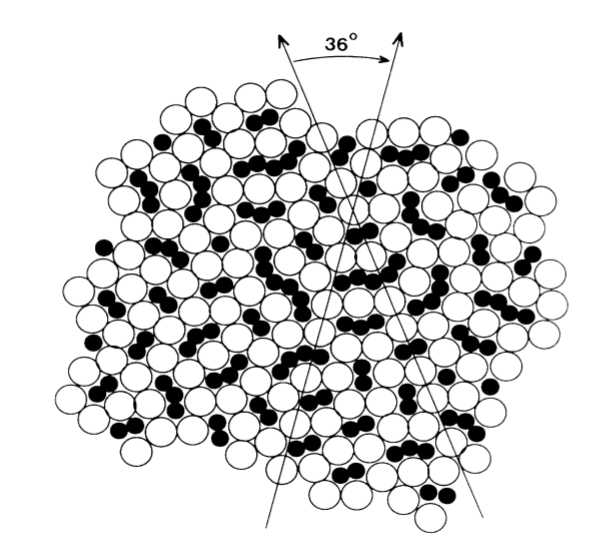
\includegraphics[width=0.5\textwidth]{10fold.PNG}
    \caption{文献\cite{PhysRevLett.58.706}中的图1,二成分兰纳德-琼斯势体系的低能态。注意这里黑色原子和白色原子的位置关系相比彭罗斯镶嵌更加“随意”,没有明确的镶嵌规则。}
    \label{fig:10fold}
\end{figure}

\section{准晶的生长}\label{sec:growth}

在说明了理论上确实可以存在稳定的准晶序之后,我们讨论准晶生长的动力学过程。对动力学过程的研究是非常重要的,因为实际的凝聚态系统中充斥着各种亚稳态和寿命较长的瞬态\cite{PhysRevB.75.064107},一些诸如玻璃化的重要物理现象本质上就是动力学的\cite{mct-primer}。
原则上,对结晶的研究完全可以通过分子动力学模拟实现,但由于计算资源的限制,能够模拟的时间和空间尺度都极其受限\cite{PhysRevLett.88.245701}。因而,现实的准晶生长的动力学必定需要一些低能有效模型。
动态密度泛函理论是一种常见的理论框架\cite{pfc2009,PhysRevB.75.064107},其中系统的自由能被写成系统密度场的泛函,形如
\begin{equation}
    F[\rho(\boldsymbol{r})]=F_{\mathrm{id}}[\rho(\boldsymbol{r})]+F_{\mathrm{ex}}[\rho(\boldsymbol{r})]+F_{\mathrm{ext}}[\rho(\boldsymbol{r})],
\end{equation}
其中
\begin{equation}
    F_{\text {id }}[\rho(\boldsymbol{r})]=k_{B} T \int d \boldsymbol{r} \rho(\boldsymbol{r})\left\{\ln \left[\rho(\boldsymbol{r}) \Lambda^{d}\right]-1\right\}
    \label{eq:id-free-energy}
\end{equation}
为理想气体的自由能密度泛函,而
\begin{equation}
    F_{\text {ext }}[\rho(\boldsymbol{r})]=\int \dd^3 \boldsymbol{r} \rho(\boldsymbol{r}) V(\boldsymbol{r}, t)
\end{equation}
为外界势场和密度场的耦合,而
\begin{equation}
    {F}_\text{ex} / k_\text{B} T=-\sum_{n=2}^{\infty} \frac{1}{n !} \int \prod_{i=1}^{n} \dd^3 \boldsymbol{r}_{i} \delta \rho\left(\boldsymbol{r}_{i}\right) C_{n}\left(\boldsymbol{r}_{1}, \boldsymbol{r}_{2}, \boldsymbol{r}_{3}, \ldots, \boldsymbol{r}_{n} \right)
    \label{eq:ex-free-energy}
\end{equation}
为液体内相互作用引入的修正,其中$\var{\rho}(\vb*{r})$为$\rho(\vb*{r})$偏离均匀时密度的多少,而$C_n$为$n$点关联函数。
这三项中的参数可以第一性原理地获得。
在假定系统过阻尼、阻尼相比其它动力学过程明显很多,以及动态的系统状态仍然可以完全使用密度场刻画(而忽略流速场等其它物理量)后,可以使用郎之万方程导出密度场的运动方程\cite{pfc2009,PhysRevB.75.064107}
\begin{equation}
    \dot{\rho}(\mathbf{r}, t)=\gamma^{-1} \nabla \cdot\left[\rho(\mathbf{r}, t) \nabla \frac{\delta F[\rho(\mathbf{r}, t)]}{\delta \rho(\mathbf{r}, t)}\right].
    \label{eq:ddft}
\end{equation}
这是一个非线性的方程,通常称为动态密度泛函理论(dynamic density functional theory, DDFT),解之可获得结晶过程\cite{Neuhaus_2014},但仍然耗费较多计算资源。前一节介绍的金斯堡-朗道理论在唯象地引入动力学之后可以更加高效地模拟结晶,称为相场模型,已经在材料科学中取得了广泛应用\cite{provatas2011phase,boettinger2002phase},但一般的相场模型通常直接将周期性的密度场平滑化(如见\prettyref{fig:phase-field})到看不清其晶格结构,即假定晶相内部完全是均匀各向同性的,这会遗漏弹性各向异性、晶向等信息。
一种兼顾计算简单和物理图像完整的理论是相场晶体(phase field crystal, PFC)方法,它基于一个简化了的自由能密度泛函和将\eqref{eq:ddft}右边括号内的$\rho(\vb*{r})$用稳定时的密度替换得到的时间演化方程
\begin{equation}
    \dot{\rho}(\vb*{r}) = \gamma^{-1} \rho_0 \laplacian \fdv{F}{\rho(\vb*{r})},
    \label{eq:pfc-eom}
\end{equation}
形式上很像普通的相场理论,但是可以从动力学经典密度泛函理论推导出,且平衡时密度分布是(准)周期性的\cite{pfc2009,PhysRevB.75.064107}。

\begin{figure}
    \centering
    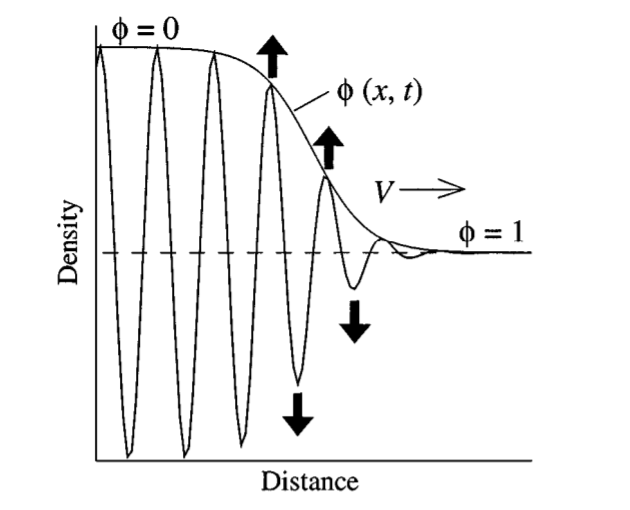
\includegraphics[width=0.4\textwidth]{phase-field.PNG}
    \caption{相场的物理解释,来自文献\cite{boettinger2002phase}中的图1,其中$\phi(x)$为相场}
    \label{fig:phase-field}
\end{figure}

\begin{figure}
    \centering
    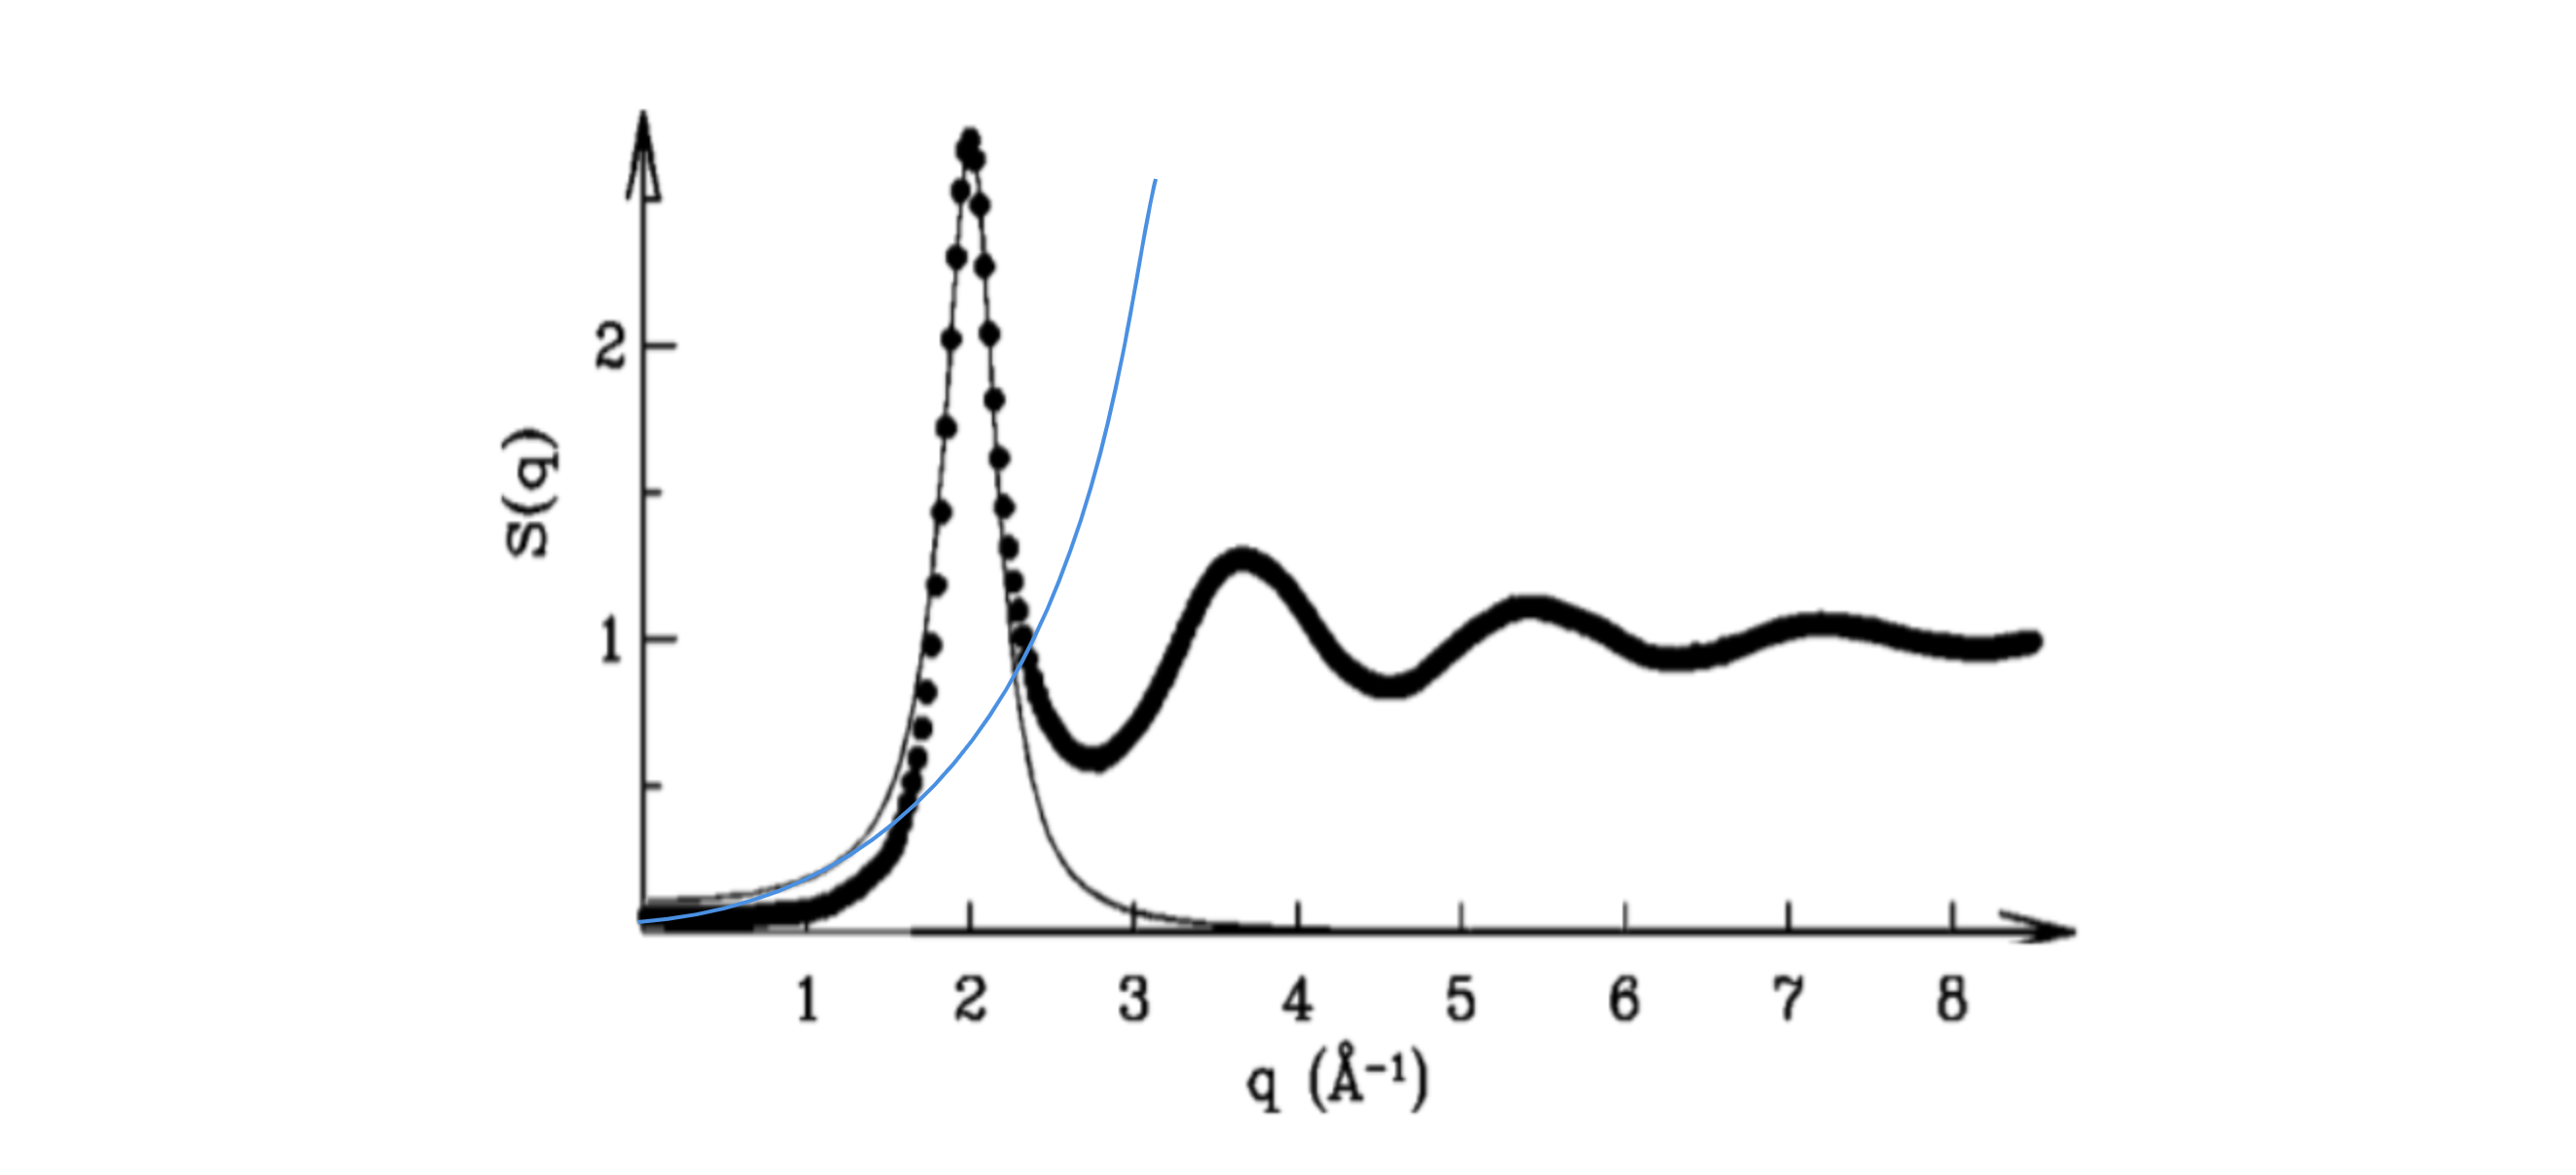
\includegraphics[width=0.6\textwidth]{sq-adapted.png}
    \caption{拟合$S(\vb*{q})$的不同方式,改编自文献\cite{PhysRevE.70.051605}的图1。蓝色曲线给出动量展开近似,黑色钟形曲线给出正态曲线近似。}
    \label{fig:sq-fitting}
\end{figure}

我们做所谓的Ramakrishnan-Yussouff近似,记
\begin{equation}
    \phi(\vb*{r}) = \frac{\rho(\vb*{r}) - \rho_0}{\rho_0},
\end{equation}
对\eqref{eq:id-free-energy}按照$\phi(\vb*{r})$做级数展开,在\eqref{eq:ex-free-energy}中仅仅保留$\phi^2$项,即仅仅保留
\begin{equation}
    F_\text{ex} = - \frac{k_\text{B} T \rho^2_0}{2} \int \dd[3]{\vb*{r}} \int \dd[3]{\vb*{r}'} {\phi(\vb*{r})} C_2(\vb*{r}, \vb*{r}') {\phi(\vb*{r}')}, 
\end{equation}
并对$C_2$(实际上就是结构因子$S(\vb*{q})$的傅里叶逆变换)做波矢展开,即
\begin{equation}
    C_2 = C_{20} + C_{22} \laplacian + C_{24} \nabla^4 + \cdots,
\end{equation}
或者也可以用正态曲线来拟合$C_2$的低波矢部分。不同的拟设形式拟合了$S(\vb*{q})$的不同行为,波矢展开相当于拟合了$q=0$到第一个峰的部分,正态曲线相当于拟合了第一个峰。对这些拟设形式的直观展示见\prettyref{fig:sq-fitting}。
该近似最早由Ramakrishnan和Yussouff导出\cite{PhysRevB.19.2775,Singh1991351},我们这里展示的是其较为现代和清楚的形式\cite{pfc2009}。
通常我们不会引入$\phi$的高阶项,因为按照重整化群理论,$\phi$的高阶项一般都是irrelevant的\cite{kardar2007statistical}。
高阶$\nabla$项虽然也是irrelevant的,从而在一般的统计场论中也会被忽略,但是在PFC中是必要的,因为需要它们来引导周期性或准周期性结构形成(直观地看,一般的统计场论分析的都是重整化群不动点附近的行为,周期性结构的波矢总是有限的,但是我们关心的空间尺度的倒数可以任意的小,从而在重整化群不动点附近,密度场的周期性结构的细节将被抹去;在PFC理论中我们需要把高阶$\nabla$项找回来以重新获得周期性结构)。
一个简单的适用于晶体形成的示例由\cite{PhysRevLett.88.245701}给出,在适当地做无量纲化之后,能够得到
\begin{equation}
    F = \int \dd^3 \boldsymbol{r}\left\{\psi\left[\left(q_{0}^{2}+\nabla^{2}\right)^{2}-\epsilon\right] \psi / 2+\psi^{4} / 4\right\},
    \label{eq:swift-hohenberg-free-energy}
\end{equation}
其中$\psi$是无量纲化的$\phi$;按照统计场论中通常的情况,$\epsilon$反映了温度\cite{kardar2007statistical}。按照\cite{PhysRevE.70.051605}中的方法引入拟设$\psi(\vb*{r}) = A \cos(\vb*{q} \cdot \vb*{r})$,会发现\eqref{eq:swift-hohenberg-free-energy}的$\psi$二阶项成为
\[
    F_2 \propto (q_0^2 - \vb*{q}^2)^2 - \epsilon.
\]
我们发现$\abs*{\vb*{q}}^2 = q_0^2$是一个极小值点,即\eqref{eq:swift-hohenberg-free-energy}诱导了一个波矢长度大体上在$q_0$附近的周期性序形成;如果我们在\eqref{eq:swift-hohenberg-free-energy}中仅仅考虑$\nabla^2$阶的导数,那么只有
\[
    F_2 \propto q_0^2 - \abs*{\vb*{q}}^2,
\]
即没有极小值点,没有稳定的周期性结构生成。根据\eqref{eq:swift-hohenberg-free-energy}和\eqref{eq:pfc-eom}可以得到无量纲化的运动方程
\[
    \pdv{\rho}{\tau} = \laplacian ((- \epsilon + (1 + \laplacian)^2) \psi + \psi^3),
\]
或者更常见的,引入一个无平均的随机扰动$\eta$以唯象地描述热涨落并改善方程的解析行为\cite{PhysRevLett.88.245701}:
\begin{equation}
    \pdv{\rho}{\tau} = \laplacian ((- \epsilon + (1 + \laplacian)^2) \psi + \psi^3) + \eta.
\end{equation}
这个方程称为Swift-Hohenberg方程,在一般的PFC出现之前由Swift和Hohenberg在研究流体动力学涨落时导出\cite{PhysRevA.15.319},是著名的模式形成方程\cite{phasediffusion2012},已经被用于计算成核、晶体生长、稳定相等结晶学问题\cite{PhysRevLett.88.245701,PhysRevE.70.051605}。% https://www.chem.uci.edu/~lawm/Lowengrub%2010-14-10.pdf

\begin{figure}
    \centering
    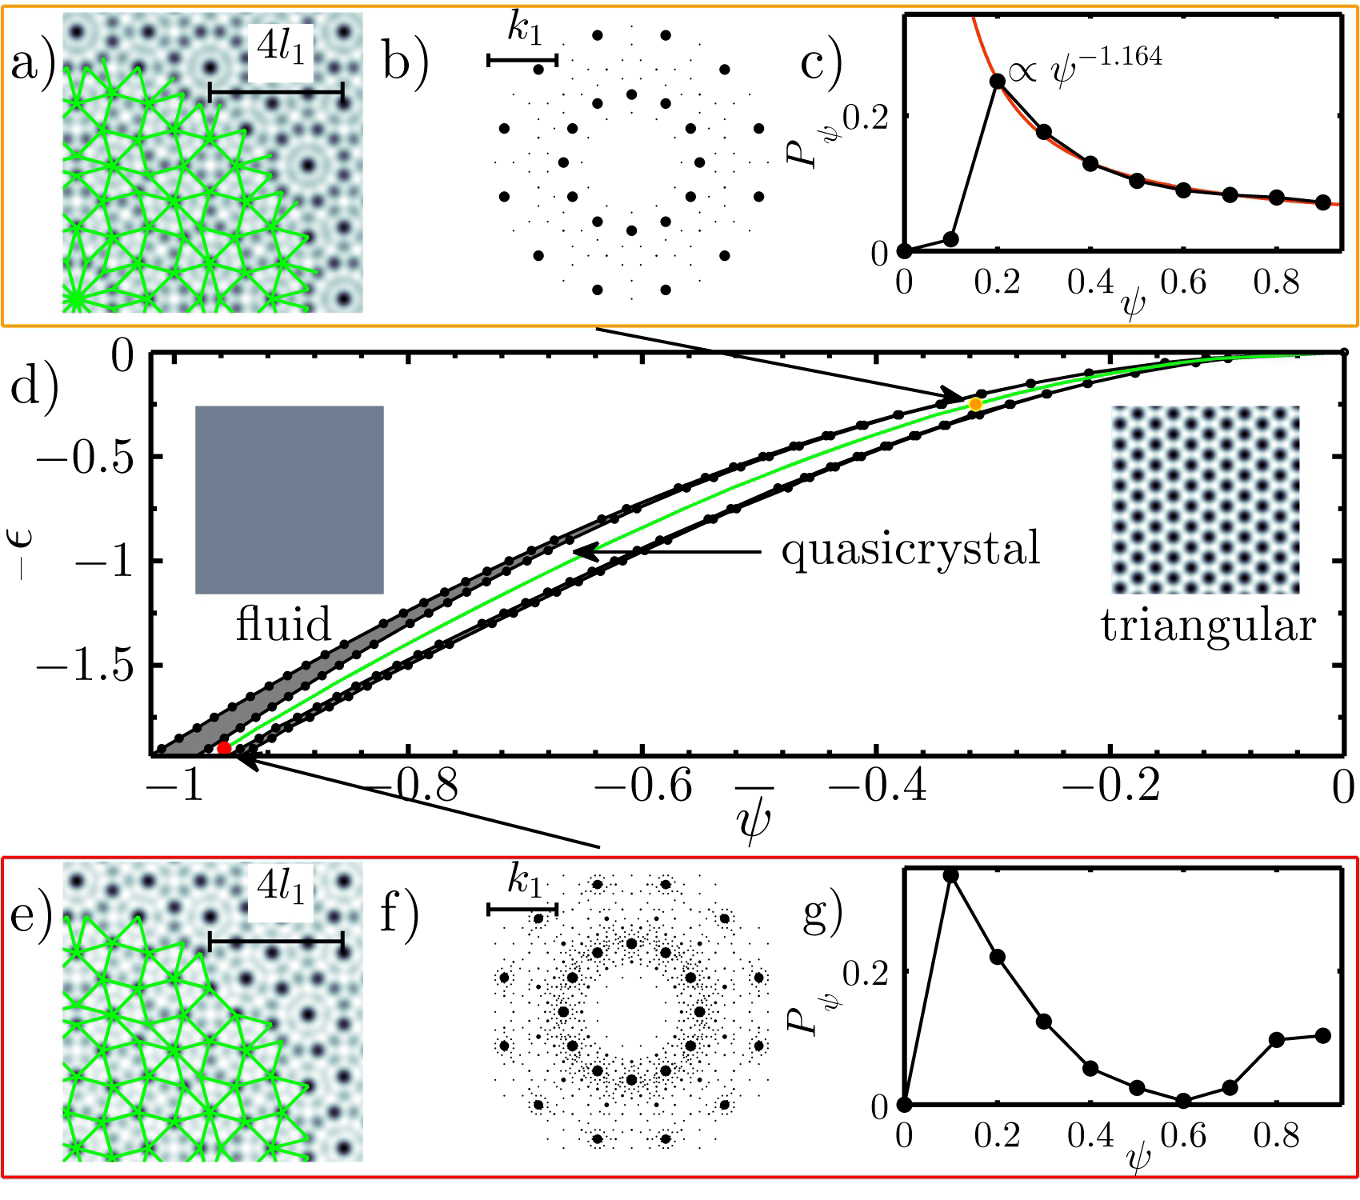
\includegraphics[width=0.8\textwidth]{phase-diagram.png}
    \caption{使用演化方程\eqref{eq:generalized-sh},取$k = 2 \cos(\pi / 12)$时的相图,取自文献\cite{PhysRevLett.112.255501}图1。}
    \label{fig:phase-diagram}
\end{figure}

\begin{figure}
    \centering
    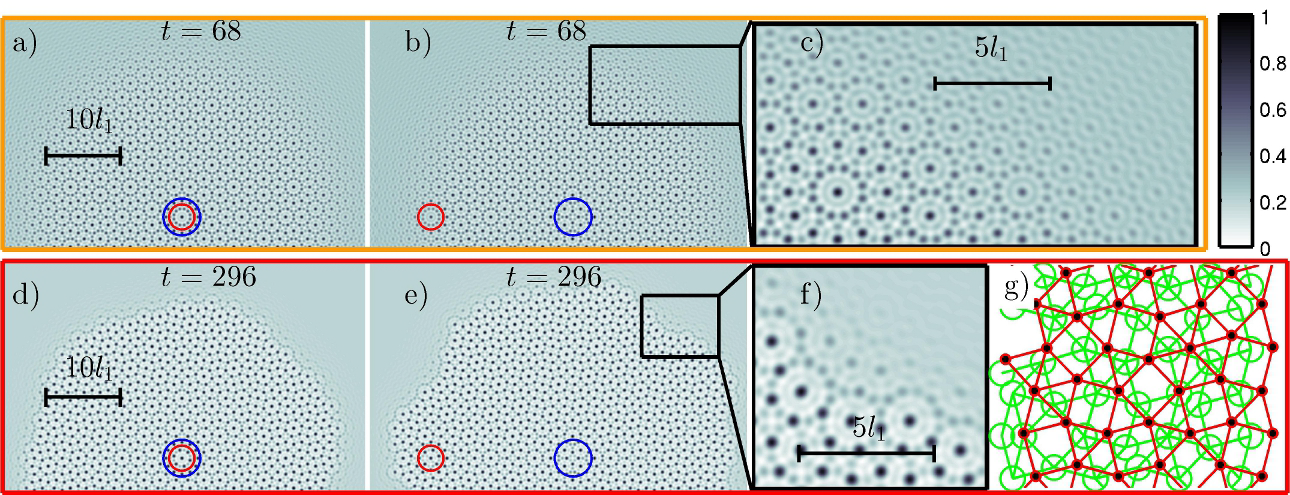
\includegraphics[width=0.8\textwidth]{growth.png}
    \caption{使用演化方程\eqref{eq:generalized-sh},取$k = 2 \cos(\pi / 12)$时准晶的生长情况,取自文献\cite{PhysRevLett.112.255501}图2。(a), (b), (c), (d)四张图排成的矩阵中,第一行来自\prettyref{fig:phase-diagram}(d)中的橙色点,第二行来自\prettyref{fig:phase-diagram}(d)中的红色点,第一列展示了晶种中心(用蓝圈圈出)也是整块准晶的全局对称中心(用红圈圈出)的情况,第二列展示了晶种中心不是全局对称中心的情况。}
    \label{fig:evolution}
\end{figure}

我们只需要将\eqref{eq:swift-hohenberg-free-energy}略加修改,就能够使用和描述晶体形成完全一致的方式描述准晶形成。文献\cite{PhysRevLett.112.255501}考虑了一个二维液体,并在$C_2$中引入更高阶波矢分量,将\eqref{eq:swift-hohenberg-free-energy}扩展为
\begin{equation}
    \pdv{\rho}{\tau} = \laplacian((- \epsilon + (k^2 + \laplacian)^2 (1 + \laplacian)^2) \psi + \psi^3).
    \label{eq:generalized-sh}
\end{equation}
当$k$很大时,重新无量纲化,上式就回退到\eqref{eq:swift-hohenberg-free-energy}。可调参数包括实际上代表了温度的$\epsilon$,平均密度$\bar{\psi}$,以及长度尺度$1 / k$。如果要生长出正方形,考虑到正方形在边的方向上和对角线的方向上均为周期性的,比较好的选择是令$k = \sqrt{2} / 2$,以保证这种周期性结构自由能较低;类似的,要生长出十二边形对称性的准晶,则应该设置$k = 2 \cos(\pi / 12)$。如此设置之后,考虑平衡态可以得到相图\prettyref{fig:phase-diagram}。
可以看到,有流体相,几乎和使用Swift-Hohenberg方程计算出来的结构毫无差别、晶格常数和$k$无关的三角晶格相,准晶相,以及用灰色标记的共存相。然而,\prettyref{fig:phase-diagram}(d)中观察准晶相的参数空间中用橙色和红色标出的两点的准晶状态,可以观察到明显的不同:\prettyref{fig:phase-diagram}(d)中的橙色点温度较高(从流体相在上、晶体相在下可以看出\prettyref{fig:phase-diagram}(d)上部为高温区),其实空间密度场$\rho(\vb*{r})$(见\prettyref{fig:phase-diagram}(a))相比于红色点的$\rho(\vb*{r})$(见\prettyref{fig:phase-diagram}(e))有更加清晰的结构。
类似的情况也出现在倒空间中,或者说出现在衍射图样中:可以看到\prettyref{fig:phase-diagram}(b)明显比\prettyref{fig:phase-diagram}(f)明锐,后者有杂乱的峰。
这种差别可以通过观察准晶化过程得到理解。\prettyref{fig:evolution}中(a), (b), (c), (d)四张图是在\prettyref{fig:phase-diagram}中的低温红色点和高温橙色点上使用不同的晶种作为初始构型计算得到的,(a)和(d)中晶种是围绕着一块理想准晶的全局对称中心(绕着该点可以看到一个非常完美的12重旋转对称性)切割下来的,而(b)和(e)中晶种中心不是全局对称中心。
可以看到,高温处,准晶的边界形状是各向同性的,准晶-液体过渡区是比较宽的,而低温时准晶的边界形状是各向异性的,准晶-液体过渡区是非常窄的,边界就是一些准晶镶嵌中的圈状结构(文献\cite{PhysRevLett.112.255501}中称为flower),缺乏高温处大致形成了准晶结构但不甚清楚的边界。
由于低温形成三角晶格时$k$的值并不重要,文章推测上述现象来自低温时边长为$l_1 = 2\pi$而非$l_2 = 2\pi / k$的结构更容易形成,从而在准晶-液体界面处,如果一个直径大体为$2l_1$的flower能够形成,它会立刻被形成。其结果是这样形成的准晶并不是自由能最优化的,并且与该flower相邻的flower将发生一定扭转和位置重排才能够让准晶继续往外扩张,从而在准晶中引入固化的局域phason(准晶中对应于原子位置局部重排的一种元激发)。
由于phason的弛豫要明显更慢,它们可以长时间存在\cite{PhysRevB.32.7444},成为一种缺陷,从而低温时形成的准晶的结构由于到处存在的phason而和理想的自由能最低的准晶相差甚远。这导致了\prettyref{fig:evolution}中(b)和(e)的一个明显对比:温度较高的(b)的晶种虽然不含有全局对称中心,但是随着准晶生长能够产生一个全局对称中心(用红色圈标出),而(e)却不能够在本应出现全局对称中心的同样位置产生全局对称中心(可以看到\prettyref{fig:evolution}(e)中被红圈圈出的地方和(b)有明显区别)。
同样的机制也可能导致了低温时准晶-液体边界更加窄、各向异性,因为并非边界上的每一个地方都能够均匀地即刻向外无限制地扩张。
对周期性的普通晶体,也存在结晶时温度过低导致能量并非最优的晶体结构容易生成,反而会引入更多缺陷的现象\cite{2018fox},但是普通结晶中显然是没有phason的。以上对准晶形成的动力学研究展示了准晶独有的生长和缺陷形成方式。

\begin{figure}
    \centering
    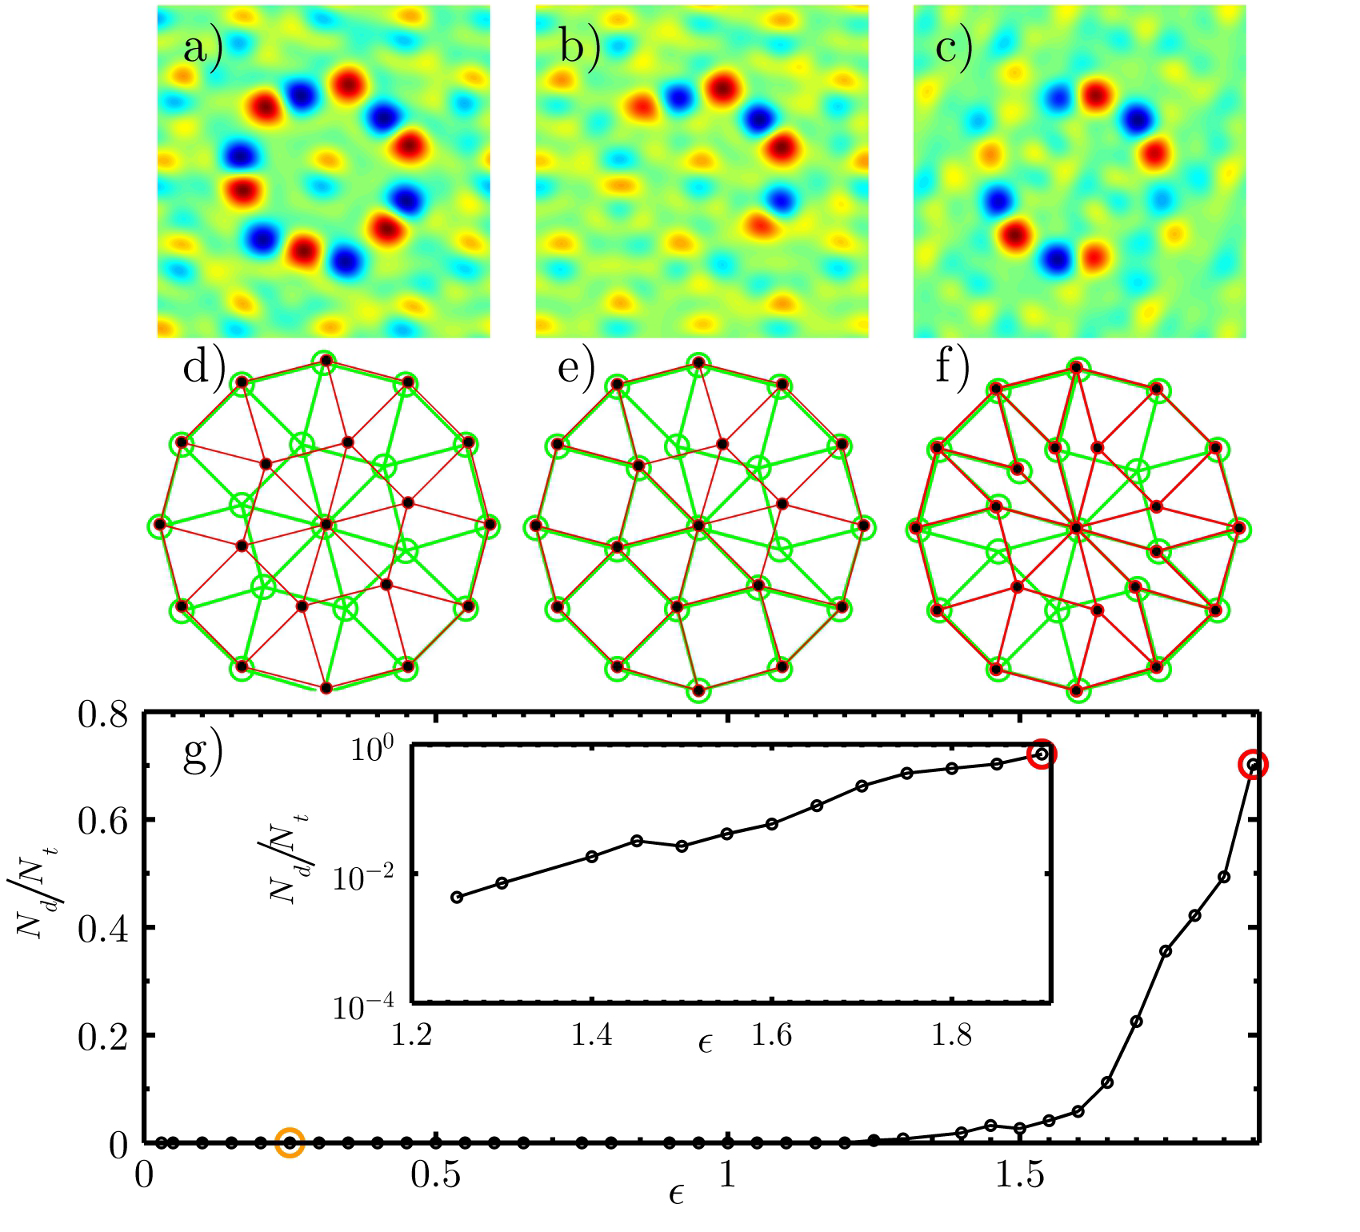
\includegraphics[width=0.5\textwidth]{phason.png}
    \caption{常见的phason构型和其数量随温度变化的趋势,取自文献\cite{PhysRevLett.112.255501}中的图3。(a), (b)和(c)是实际计算得到的密度场减去自由能最优化的准晶密度场得到的结果,(d), (e), (f)给出出现phason后,实际的构型(红色)相比理想的构型(绿色)发生的畸变}
\end{figure}

\section{准晶中的电子结构}\label{sec:electron}

准晶虽然经常被划分到软凝聚态研究课题中,但是在硬凝聚态方面也有重要的意义,因为准晶常常使用合金实现,从而内部可以有大量较自由的电子。
到目前为止,我们都只是在讨论准晶的结构,而将电子视为提供原子间等效相互作用的中间媒介。但正如传统固体物理中,晶格为库仑相互作用电子气提供了周期性背景一样,准晶为电子提供了由不可公度的频率成分构成的非周期性背景。
准晶没有严格的周期性意味着无法使用Bloch定理,从而无法简单地将晶格动量、布里渊区、能带等理论推广到准晶中的电子态上。
在诸如转角石墨烯等结构上也存在这种由不可公度的频率成分构成的背景,研究准晶中的电子态从而有很大的普遍意义。

实验研究表明,一些合金制成的准晶(如GaMgZn, AlCuLi, AlCuFe, AlCuRu)中,费米能级附近的态密度很低,另一些准晶(如AlCu (Mg, Li)和(Al, Ga)MgZn)虽然有着几乎是自由电子的态密度,但是电导率反常地低,几乎是半导体的量级\cite{quasi-experimental}。这可以使用如下论证加以解释。
暂时忽略电子间的库伦排斥,如果固体中原子形成了一个波矢为$\vb*{G}$的周期性序,则动量为$\hbar\vb*{k}$的电子可以被散射到动量$\hbar (\vb*{k} + \vb*{G})$上;如果碰巧这两个动量的电子能量接近,这两个电子模式就会发生强烈的耦合,从而在$\hbar^2 \vb*{k}^2 / 2m$能量附近打开能隙,体现在动量空间中,就是$\vb*{G}$的垂直平分线两侧电子能量发生跃变。
在晶体中,由于可能的$\vb*{G}$形成倒格子,动量空间将被分割成第一布里渊区及其平移后的复制品,对应一条条能带,每条能带内部能量连续分布,电子态都是连续延展的、类似于平面波;但是在准晶中,所有可能的$\vb*{G}$是稠密的,似乎动量空间将被非常细碎地分割。这似乎暗示准晶中的电子态不可能是延展态,而是局域的。
然而,ARPES实验能够观察到非常像是能带色散关系的结构,这可能是由于部分$\vb*{G}$对应的准晶原子势场实际上很弱,从而电子可以被认为仅仅被有限个$\vb*{G}$分量散射了,从而仍然近似可以认为存在能带\cite{ROTENBERG2004237}。
此外,虽然缺乏良定义的布里渊区和费米面,但理论上可以导出,准晶中的电子在磁场作用下同样可以发生de Haas-van Alphen效应,如果唯象地将$\vb*{k}$划过的曲面看成“赝”费米面,得到的费米面将具有非平庸的拓扑性质,且类似的现象在特定角度的转角石墨烯中也存在\cite{PhysRevB.100.081405}。
一些拓扑物态,包括量子霍尔效应、量子反常霍尔效应、量子自旋霍尔效应、拓扑绝缘体等也已经被移植到了准晶背景下\cite{topo2021}。

\section{结论}

对准晶的形成和其中电子行为和研究和整个凝聚态物理的其他部分均有密切联系。分析准晶稳定性的金斯堡-朗道理论是处理对称性相关的相变的统一范式。
研究准晶形成的相场方法和PFC方法揭示了准晶相比普通晶体的特别之处、不同参数下的生长情况,也与材料学上对结晶行为的数值模拟共享理论框架,且是模式形成等偏微分方程和非线性系统中的数学议题的物理动机之一。
准晶中的电子行为扩展了硬凝聚态物理对电子结构的研究,并且和眼下热门的转角石墨烯乃至其它转角二维材料中的电子态类同。准晶背景也可能能够容纳新的新奇拓扑物态。

\bibliographystyle{plain}
\bibliography{main} 

\end{document}